\section{Experiments and Results}
\label{sec:eval}
We use kaggle dataset available at AmExpert 2019. Figure \ref{fig:data} shows the schema of the data we have used 
to build our models. As mentioned in Section \ref{sec:methodology}, we use a maximum of 1 year data aggregated at bi-weekly 
level at consumer-item granularity. We split the data into three part train, validation and test based 
on our validation strategy. We generate consumer - item - bi-weekly data with purchase/ non purchase 
being the target , and use this data to train all our models.
  \begin{figure}[hbt!]
    \centering 
    \caption{Exploratory Data Analysis} 
    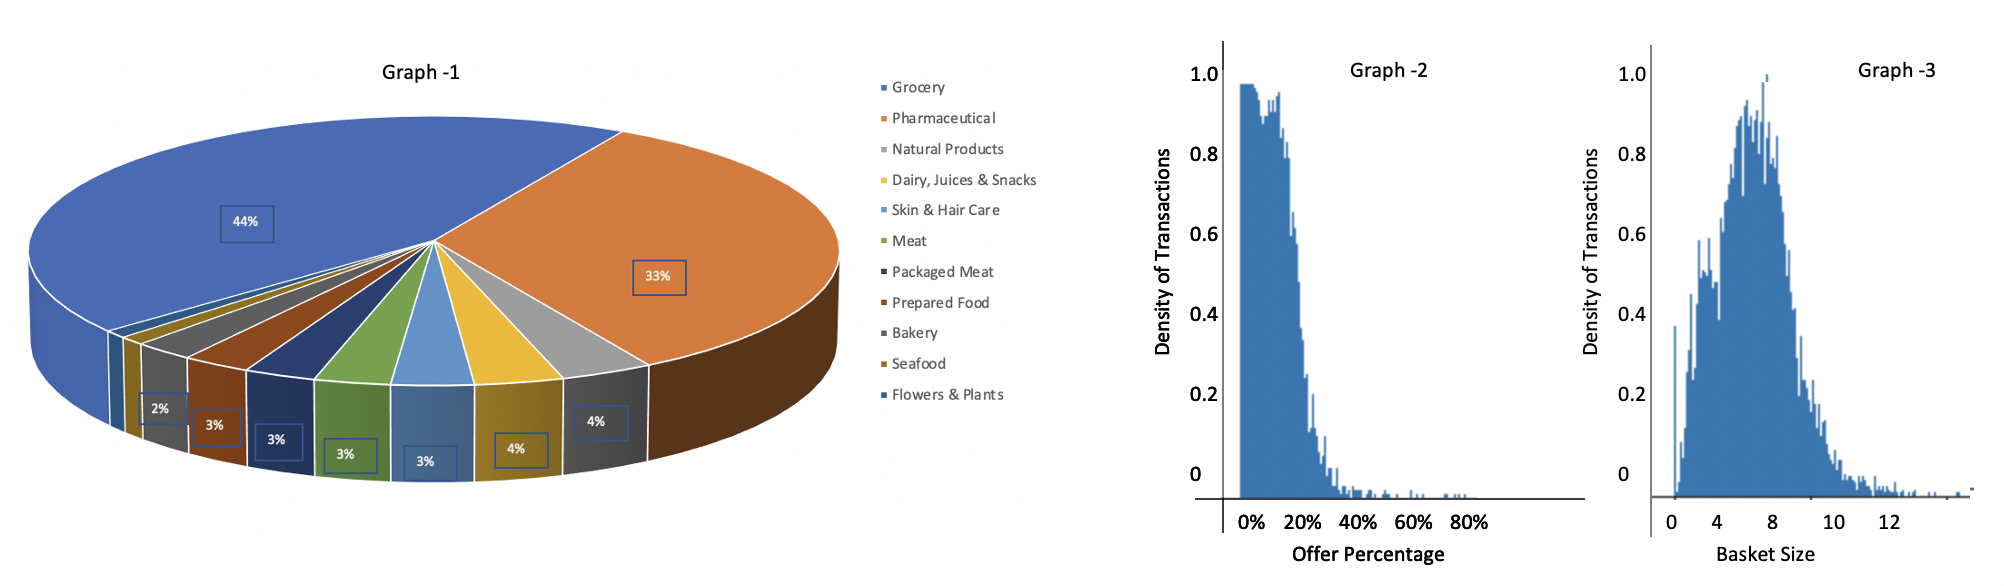
\includegraphics[width=5.5in]{img/sales_dist.png} 
    \label{fig:sales_dist} 
  \end{figure}
  \subsection{Experiment Setups}
We start with exploratary data analysis, looking at the data from various cuts. We
study the variations of different features with our target (purchase/ non purchase). Some of our studies include
category-wise sales distribution, density of transactions with varying offer percent 
and density of transactions with varying basket size (Figure~\ref{fig:sales_dist}).
We observe that Grocery and Pharmaceutical contributes to ~77% of total sales.
We also look at order probability variations at different temporal cuts like week, month and quarter, transactional metrics 
like total orders, total reorders, recency, gap between orders, at both consumer and item levels.
We then perform multiple experiments with the above mentioned features and different hyperparameter 
configurations to land at reasonable hyperparameters to perform final experiments and present our results.
  \begin{figure}[hbt!]
    \centering 
    \caption{Category graphs} 
    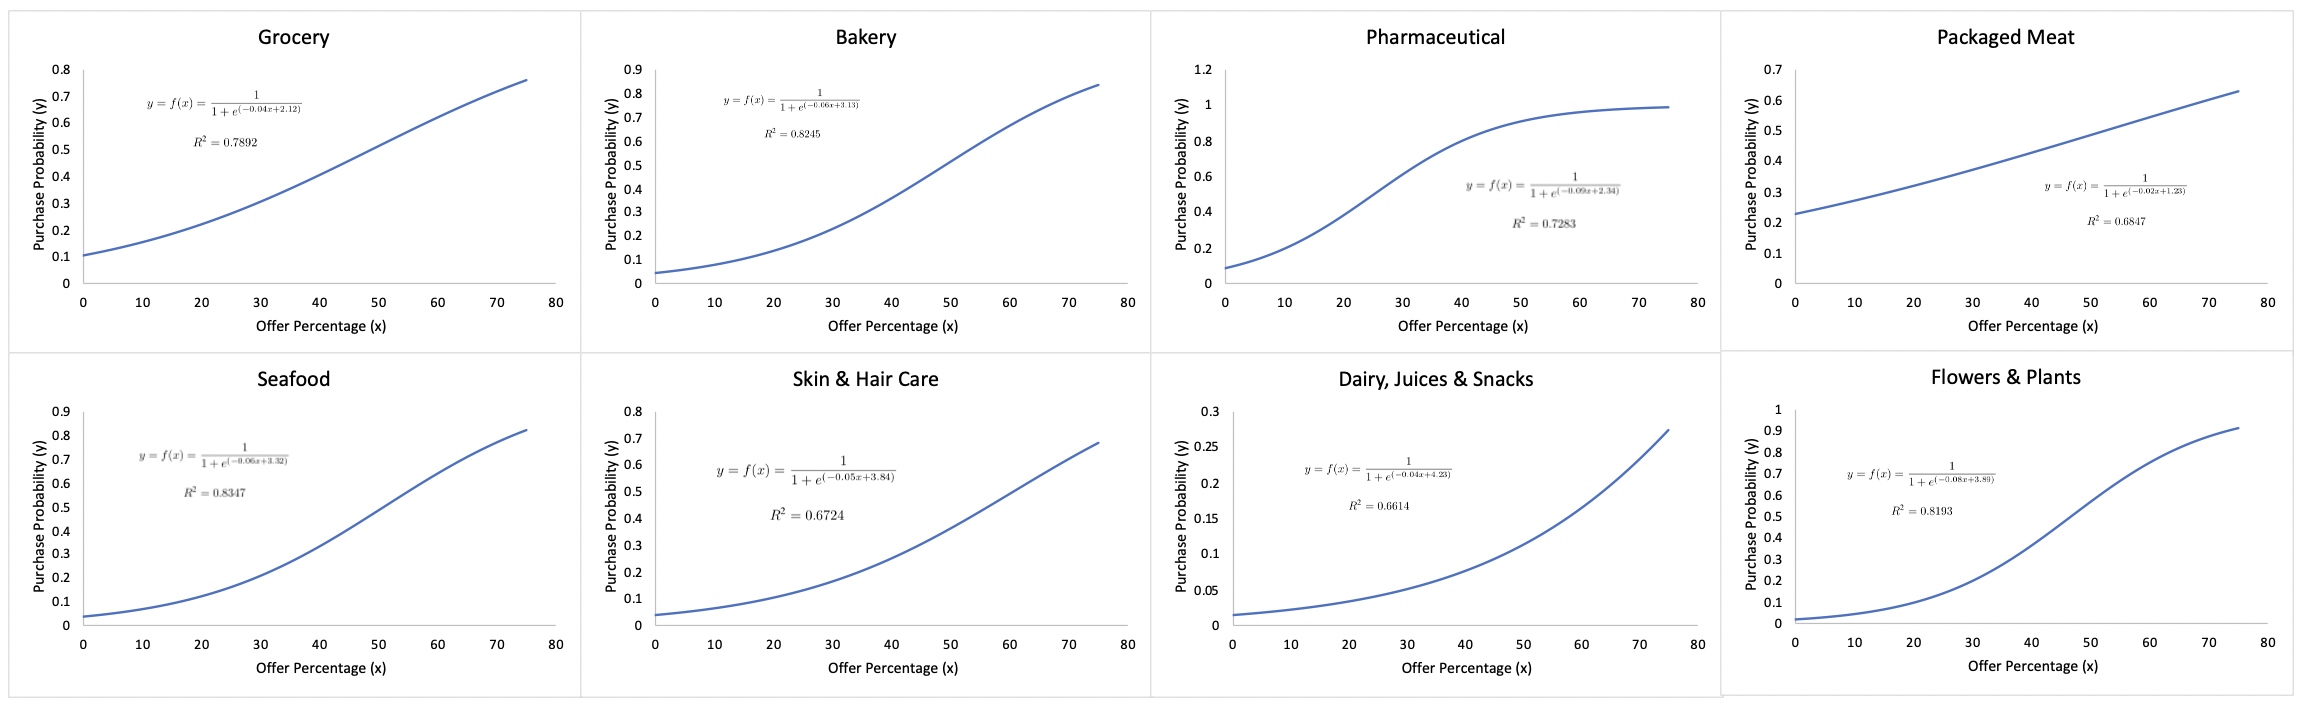
\includegraphics[width=5.5in]{img/cat_curves.png} 
    \label{fig:cat_curves} 
  \end{figure}
 \begin{figure}[hbt!]
    \centering 
    \caption{Probability Distributions} 
    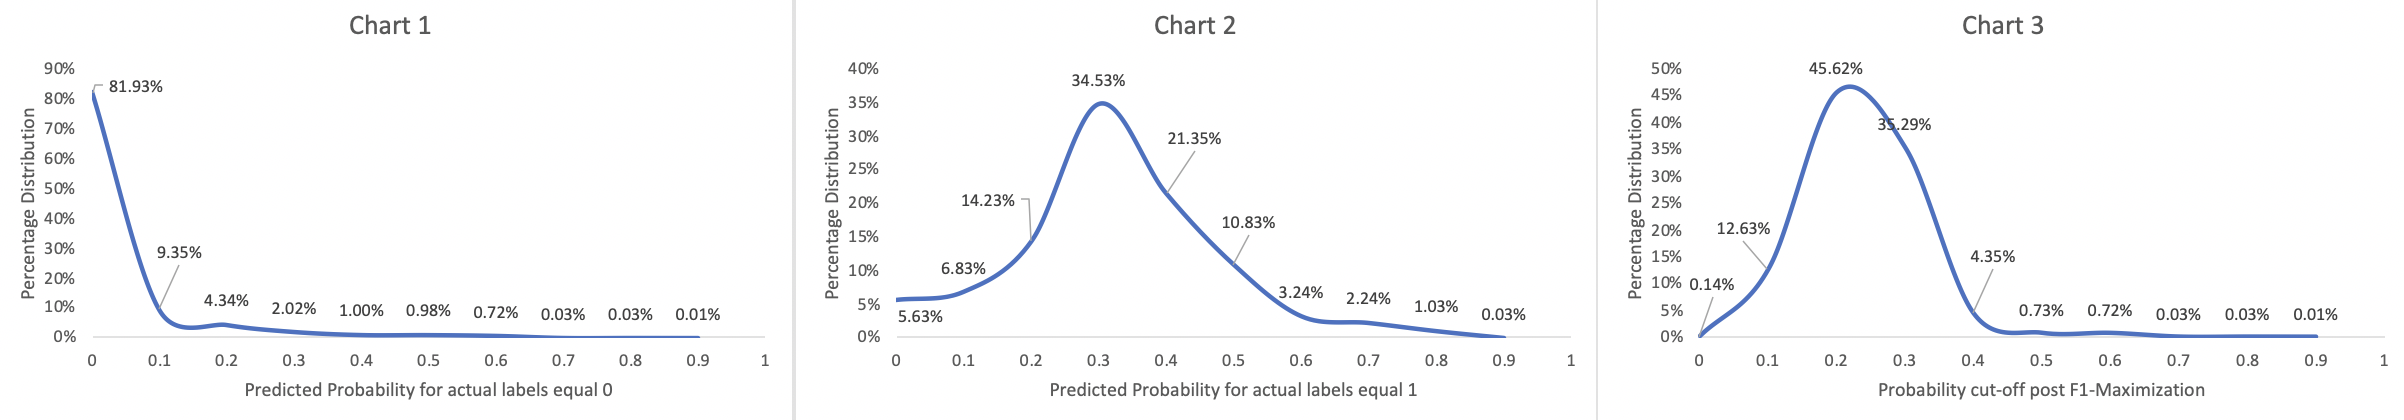
\includegraphics[width=5.5in]{img/prob_dist.png} 
    \label{fig:prob_dist} 
  \end{figure}
\subsection{Results and Observations}
Figure \ref{fig:cat_curves} shows the functional relationship of offer percetage with purchase probability 
obtained across different categories. It also contains the equations and goodness of fit in the 
form of R\textsuperscript{2} for each category. Seafood and Bakery are the top 2 best fitted categories
with R\textsuperscript{2} values of 0.83 and 0.82 respectively. Figure \ref{fig:prob_dist} Chart-1 and Chart-2 shows the 
predicted probability distributions of actual label equals 0 and 1 respectively over the validation data split.
Chart-3 shows the cut-off probability distribution post F\textsubscript{1}-Maximization, and, we observe 
that highest density of cut-off probability lies between 0.2 to 0.3. Table \ref{tab:model_results} presents the 
accuracy values post Modelling and F\textsubscript{1}-Maximization. It also has the average elasticity values 
along with weighted offer percent computed post optimization. From model performance perspective
, it is observed that Grocery category has least BCELoss of 0.0283. Pharmaceutical and Meat categories
followed Grocery with BCELoss of 0.0296 and 0.0299 respectively. Also, Grocery has the best
F\textsubscript{1} score of 0.512 followed by Meat and Pharmaceutical scoring 0.511 and 0.509
respectively. Vegetables is the most elastic category with elasticity value of 1.53, whereas 
Packaged meat and Skin and Hair care are the least elastic categories with elasticity value of 0.62.
From Figure \ref{fig:optimize}, we can see the graphical representation of distribution of 
optimal offer calculated through optimization. We find Skin and Hair care along with Pharmaceutical to be 
left skewed, whereas Vegetables as well as Flowers and Plants to be right skewed.
 \begin{figure}[hbt!]
    \centering 
    \caption{Optimal Offers} 
    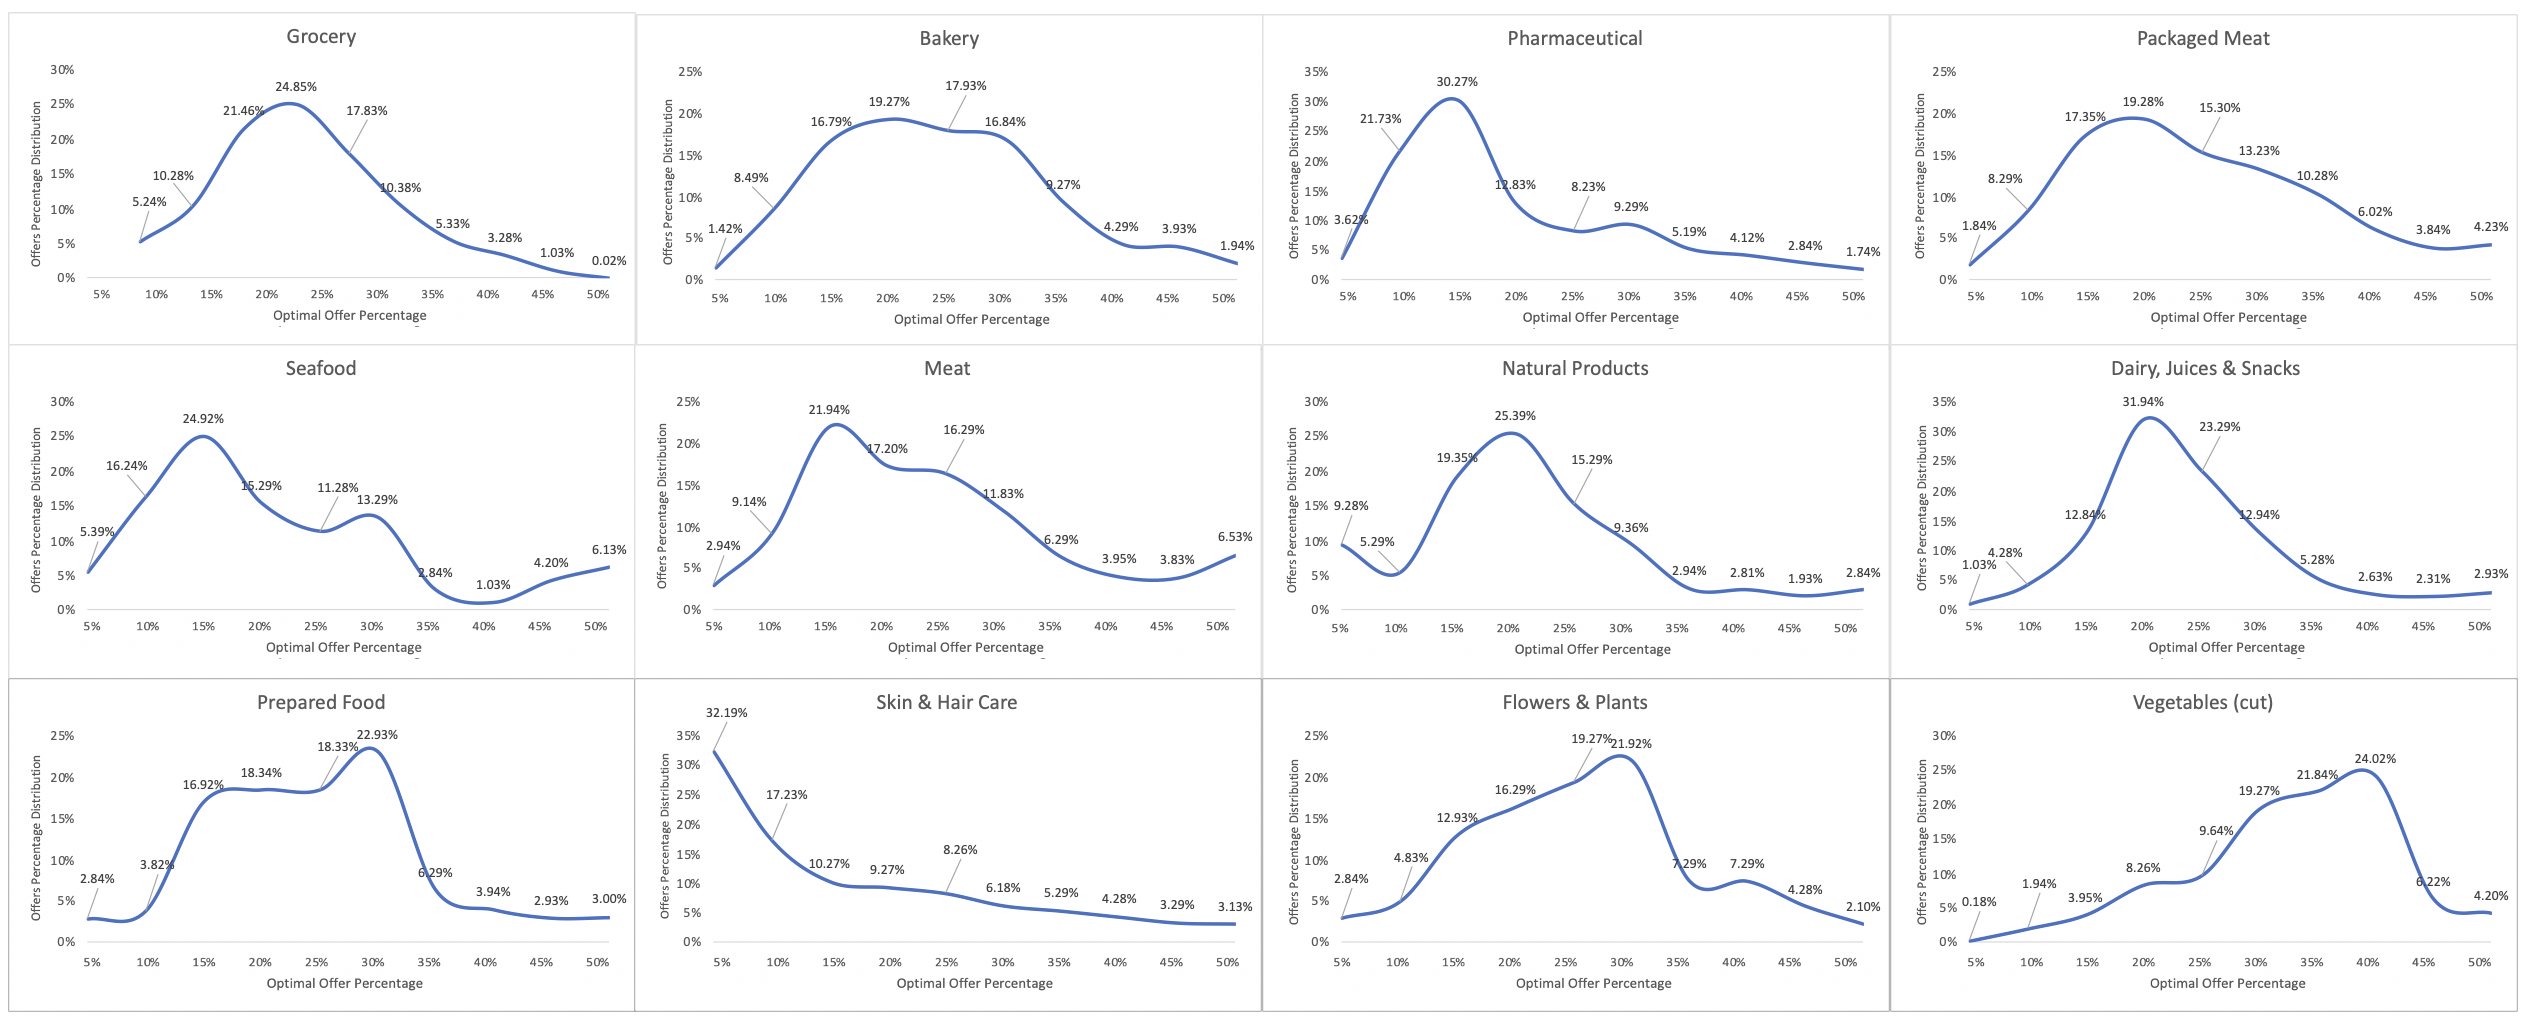
\includegraphics[width=5.5in]{img/optimize.png} 
    \label{fig:optimize} 
  \end{figure}
\begin{center}
\begin{table*}[hbt!]
\caption{Model Results and Elasticity} 
\centering
\resizebox{\textwidth}{!}{\begin{tabular}{|l|c|c|c|c|c|c|c|}
\hline
{\bf Category} & {\bf Sample size} & {\bf BCELoss} & {\bf Precision} & {\bf Recall} & {\bf F\textsubscript{1}-Score} & 
{\bf Avg Elasticity} & {\bf Weighted Offer Percent} \\
\hline\hline
Grocery  		&  28,990 &  0.0283 & 0.524 & 0.501 & 0.512 & 1.13 & 23.37\\ \hline
Bakery  		&  1,628 &  0.0415 & 0.346 & 0.391 & 0.367 & 1.06 & 22.15 \\ \hline
Pharmaceutical  		&  20,492 &  0.0296 & 0.538 & 0.483 & 0.509 & 0.73 & 17.89 \\ \hline
Packaged Meat  		&  1,473 &  0.0329 & 0.473 & 0.452 & 0.462 & 0.62 & 19.15 \\ \hline
Seafood  		&  539 &  0.0382 & 0.497 & 0.379 & 0.43 & 0.89 & 16.23\\ \hline
Natural Products  		&  2,399 &  0.0319 & 0.451 & 0.524 & 0.485 & 0.95 & 21.78 \\ \hline
Dairy, Juices, Snacks  		&  2,060 & 0.0396 & 0.394 & 0.492 & 0.438 & 1.04 & 22.02\\ \hline
Prepared Food  		&  1,407 &  0.0472 & 0.338 & 0.295 & 0.315 & 1.03 & 28.27 \\ \hline
Skin, Hair Care  		&  1,906 &  0.0391 & 0.429 & 0.453 & 0.441 & 0.62 & 7.93 \\ \hline
Meat  		&  1,767 &  0.0299 & 0.498 & 0.524 & 0.511 & 0.94 & 18.92\\ \hline
Flowers, Plants  		&  491 & 0.0483 & 0.275 & 0.318 & 0.295 & 1.43 & 30.24 \\ \hline
Vegetables (cut)  		&  124 &  0.0469 & 0.364 & 0.267 & 0.308 & 1.53 & 37.92\\
\hline
\end{tabular}}
\label{tab:model_results}
\end{table*} 
\end{center}
\subsection{Industrial Applications}
Offer Personalization framework has multiple applications in the retail industry. Some of them 
include: {\bf Personalized Marketing:} Optimal offer rollouts can be made at consumer-item granularity. 
{\bf Inventory Planning:} Consumer preference model used to compute optimal offers can also be used in better 
short term inventory planning (2-4 weeks), which is largely dependant over what consumer is going to purchase in the near future.